\begin{frame}{Beispiel: $H_{\mathrm{O}}$, $H_{\mathrm{OE}}$, $H_{\mathrm{OS}}$}
	\alt<1>{\begin{itemize}
		\item{Betrachtung mit je einem Freiheitsgrad für (S) und (O)}
		\begin{itemize}
			\item{Subjekt: \ketsmiley, \ketneutrey, \ketfrowny}
			\item{Objekt: \ketup, \ketdown}
		\end{itemize}
		\item{Gesamtsystem S $\otimes$ O mit 6 Basiszuständen:\\
			\ketsmileyup, \ketsmileydown,\ketneutreyup, \ketneutreydown,\ketfrownyup, \ketfrownydown}
		\item{Dichtematrix $\rho = \ketneutreyup\braneutreyup$ als Anfangszustand:\\}
			\vspace{0.2cm}
			\centering
			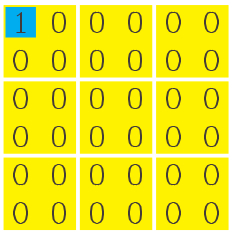
\includegraphics[scale=0.3]{graphics/subsystem_example_1_1.jpg}
	\end{itemize}}{}
		\alt<2>{\begin{itemize}
				\item{Zeitentwicklung $U = \exp(-i H_{\mathrm{O}}t)$ von $\rho_{\mathrm{O}} = \ketup\braup$}
				\begin{itemize}
					\item{$U\ketup = \frac{1}{\sqrt{2}}\del{\ketup + \ketdown}$}
					\item{Entropie bleibt konstant}
				\end{itemize}
				\end{itemize}
				\begin{columns}
					\begin{column}{0.55\textwidth}
						\begin{beamerboxesrounded}{}
							\begin{align*}
							\rho^{\prime}_{\mathrm{O}} = U\rho_{\mathrm{O}}U^{\dagger}
							=&\frac{1}{2}(\ketup\braup + \ketup\bradown \\ &+ \ketdown\braup + \ketdown\bradown)
							\end{align*}
							\vspace{-0.5cm}
						\end{beamerboxesrounded}
					\end{column}
					\begin{column}{0.35\textwidth}
						 \centering
						 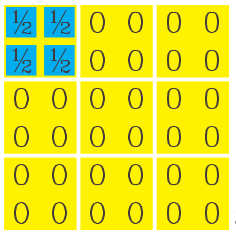
\includegraphics[scale=0.35]{graphics/subsystem_example_1_2.jpg}
					\end{column}
				\end{columns}}{}
				
		\alt<3>{\begin{itemize}
				\item{$H_{\mathrm{OE}}$: Dekohärenz (vollständig)}
				\begin{itemize}
					\item{Entropie nimmt zu}
				\end{itemize}
				\vspace{0.2cm}
				%				\centering
				%				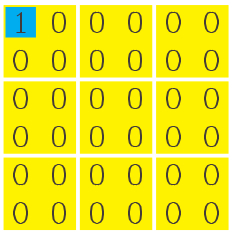
\includegraphics[scale=0.3]{graphics/subsystem_example_1_1.jpg}
			\end{itemize}
			\begin{columns}
				\begin{column}{0.55\textwidth}
					\begin{beamerboxesrounded}{}
						\begin{equation*}
						\rho^{\prime\prime}_{\mathrm{O}} = \frac{1}{2}(\ketup\braup + \ketdown\bradown)
						\end{equation*}
						\vspace{-0.5cm}
					\end{beamerboxesrounded}
				\end{column}
				\begin{column}{0.35\textwidth}
					\centering
					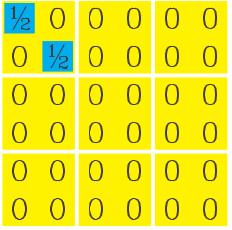
\includegraphics[scale=0.35]{graphics/subsystem_example_1_3.jpg}
				\end{column}
			\end{columns}}{}
		\alt<4>{\begin{itemize}
				\item{$H_{\mathrm{OS}}$: Messung von S an O}
				\begin{itemize}
					\item{$U = \exp(-i \int\!\!\!H_{\mathrm{OS}}\dif t)$, Messung schnell}
					\item{$U\ketneutreyup = \ketsmileyup$, $U\ketneutreydown = \ketfrownydown$}
					\item{$\rho_{\mathrm{OS}} = \ketneutrey\braneutrey \otimes \frac{1}{2}(\ketup\braup + \ketdown\bradown)$}
					\item{Entropie nimmt ab}
				\end{itemize}
				\vspace{0.2cm}
				%				\centering
				%				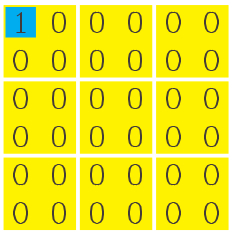
\includegraphics[scale=0.3]{graphics/subsystem_example_1_1.jpg}
			\end{itemize}
			\begin{columns}
				\begin{column}{0.55\textwidth}
					\begin{beamerboxesrounded}{}
						\begin{empheq}{align*}
						\rho^{\prime}_{\mathrm{OS}} = U\rho_{\mathrm{OS}}U^{\dagger} = &\frac{1}{2}(\ketsmileyup\brasmileyup\\ &+ \ketfrownydown\brafrownydown)
						\end{empheq}
						\vspace{-0.5cm}
					\end{beamerboxesrounded}
				\end{column}
				\begin{column}{0.35\textwidth}
					\centering
					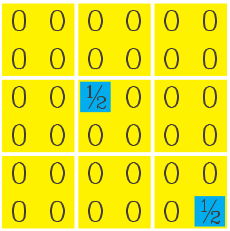
\includegraphics[scale=0.35]{graphics/subsystem_example_1_4.jpg}
				\end{column}
			\end{columns}}{}
%			\alt<5>{\begin{columns}
%					\begin{column}{0.45\textwidth}
%						\centering
%						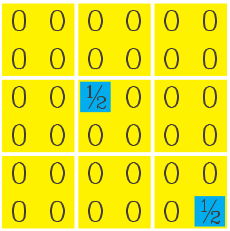
\includegraphics[scale=0.35]{graphics/subsystem_example_1_4.jpg}
%					\end{column}
%					\begin{column}{0.45\textwidth}
%						\centering
%						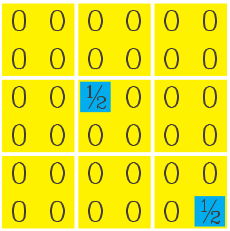
\includegraphics[scale=0.35]{graphics/subsystem_example_1_4.jpg}
%					\end{column}
%				\end{columns}}{}}{}		
\end{frame}